\section{Experiments and Results}\label{sec:experiments}

After presenting the formulation of the constraint trick we wish to test it now using an example ReLU-based network (of depth $50$, a fixed layer $N_k=4$, and a softmax output), specially targeted to (1)) fail to trivial accuracy values; (2) exhibits the highlighted issues that DNN experience (i.e, dying neurons, exploding gradient and vanishing gradient); and (3) is manageable enough to relate to analytical results such as proposed in remarks XX and XX. 
\\\\
Two datasets were used for experimentation: the \texttt{MOONS} dataset (for \emph{toying}) and the \texttt{CIFAR-10} to test in a more realistic setting involving a $5\times 5$ CNN using padding to preserve image size. Our comparison is done against batch-normalization (\emph{batchnorm} for short), that is able to overcome the problems on our network with an overall validation accuracy on the \texttt{MOONS} dataset of 60\% and in \texttt{CIFAR-10} of 56\%.  
%%%%%%%%%%%%%%%%%%%%%%%%%%%%%%%%%%%%%%%%%%%%%%%%%%%%%
%We attempt now to provide with empirical proof of the previous development. In order to do so, we use a network architecture especially targeted to highlight the problems in which a neural network can incur. We understand that if we used a normal architecture like VGG-16 or ResNet50 those problems would not arise as much and it would be more difficult to demonstrate the validity of our proposal, in addition to dealing with other mechanisms designed to solve some of the problems discusses which could interfere. Therefore, we choose the simplest architecture where using ReLU simply does not work and focus there to fix it with the hope that the results will be extrapolated in future research.

%We prepare two experiments, one using the toy dataset "moons" and another using "CIFAR-10". We aim at understanding the behavour of the parameters using a simple toy dataset and then testing in a more real-like dataset as CIFAR-10.
%The network chosen is a simple architecture composed of 50 layers of 4 units each with a softmax output. This network is used in all the experiments. In the case of CIFAR-10 we use a convolutional version of it consisting in a 5x5 convolution using padding to mantain the same image size.

%As a baseline we use ReLU which fails in all the cases, in order to show how the problem exists, and ReLU with Batch Normalization so we can compare how much our approach improves.

\subsection{Toy problem}
\paragraph{Experimental setup} We compare the performance in terms of maximum accuracy between ReLU, ReLU + Batch Normalization and SC-ReLU in the moons dataset. We sample 85 points for training and 15 for testing. The parameter grid is presented below at 
\ref{tab:grid_toy}. The results are displayed in Table \ref{tab:moons}.

\begin{table}[h]
\centering
\begin{tabular}{lr}
\hline
%\toprule
{Parameter} &         Values tested \\
%
Learning rate &  0.01, 0.001, 0.0001 \\
Batch size    &                     85 \\
Scope         &           L, U, P, U+P \\
$\lambda$          &                   0.01 \\
Epochs & 2000 \\
\hline
%\bottomrule
\end{tabular}
\caption{Parameter grid for toy experiment}
  \label{tab:grid_toy}
\end{table}

\paragraph{Accuracy} Results from Table \ref{tab:toy} show a significant improvement over the ReLU + Batch Normalization baseline. Our proposal solves perfectly the problem, whereas Batch Normalization falls significantly far at 0.6. ReLU simply fails as expected.

\begin{table}[h]
\centering
\begin{tabular}{lrrrr}
%\toprule
{} &       T. acc. &   V. acc. &      T. loss &  V. loss \\
%\midrule
Relu            &  0.517647 &      0.4 &  0.692524 &  0.693898 \\
Relu + BN     &  0.811765 &      0.6 &  0.633113 &  0.663632 \\
SP-ReLU &  1.000000 &      1.0 &  0.000063 &  0.021107 \\
%\bottomrule
\end{tabular}
\caption{Toy experiment results.}
  \label{tab:toy}
\end{table}

\paragraph{Constraint scope.} We analyze which of the many scopes used performs better using Table \ref{tab:scopes}. To our surprise the best performing variant is Layerwise which achieves perfect accuracy. We theorize this might be due the fact that the number of constraints augment on the number of points/units in which is applied, changing effectively the magnitude of the constraint loss and rendering the hyperparameter tuning ineffective. A possible solution would be to take the average instead of the sum of the constraints, in order to make it more commensurable with respect $\lambda$. One could argue that the units operating in linear regime, this is the units whose output lies in the positive quadrant for all the dataset, might play a role in the network which is not allowed by the constraints, but if that were the case Pointwise, which allow linear units, should surpass Unitwise, which does not. We leave this question for future research.

\begin{table}[h]
\centering
\begin{tabular}{lrrrr}
%\toprule
{} &       T. acc. &   V. acc. &      T. loss &  V. loss \\
Scope &           &           &           &           \\
%\midrule
L    &  1.000000 &  1.000000 &  0.000063 &  0.021107 \\
P    &  0.929412 &  0.800000 &  0.176525 &  0.647618 \\
PU   &  0.988235 &  0.933333 &  0.698847 &  1.081031 \\
U    &  0.905882 &  0.800000 &  0.416179 &  1.522891 \\
%\bottomrule
\end{tabular}
\caption{Toy experiment results by scope.}
  \label{tab:scopes}
\end{table}

\paragraph{Peakiness} Another interesting phenomena is the behavior of the constraint loss. In some cases it exhibits peaks which match accuracy improvements. Figure \ref{fig:peaks} showcases one of those cases. Note how after each of the drops the accuracy achieved improves in a way that breaks the trend followed until then. We theorize that this might be due the constraints transforming the internal arrangement of the network, by turning the hyperplanes lying inside the units located in the layers so they comply better with the separability constraints. We can see how around epoch 458 the accuracy drops to 0.21, we argue that this sudden change of accuracy is proof that one of the hyperplanes has changed its orientation. From there the constraint loss is further minimized and at iteration 710 the network starts improving again, reaching previous performance, then another peak ocurs and the network improves again in a higher rate than earlier. The same phenomena happens again but with diminished results as it approaches to what we understand that is the optimum for this set of parameters.

\begin{figure*}[h]\label{fig:peaks}
  \caption{Peaks of accuracy and constraint loss during training.}
  \centering
    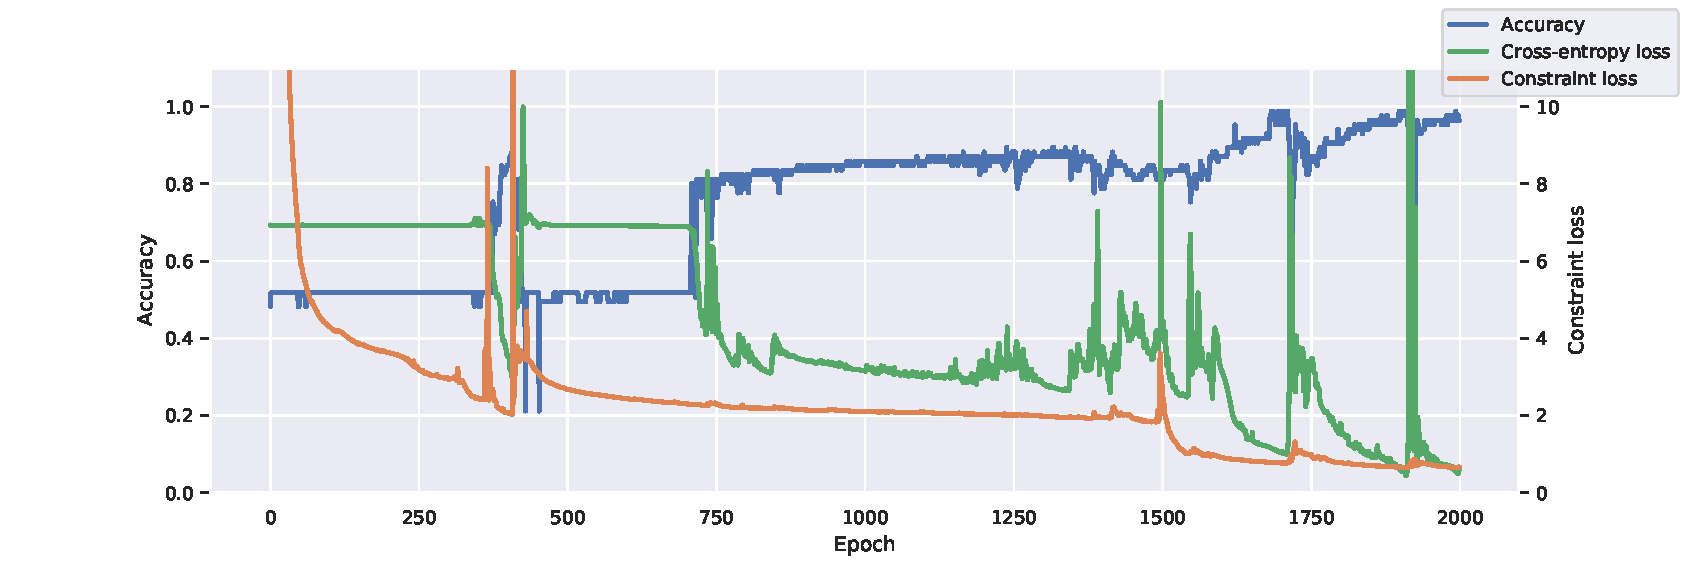
\includegraphics[width=1.0\textwidth]{peaks}
\end{figure*}

\subsection{CIFAR-10}

In order to assess our proposal with real data we apply our proposal in the CIFAR-10 dataset. We use the same network from the previous experiment but adapting the parameters to the present task, as shown in \ref{tab:grid_cifar}. Since this experiment takes longer to compute we only use the Layerwise version of our proposal, since it is the best in the previous experiment. We also tune the value of $\lambda$. Finally, since our proposal enables to train with zeros initialization we compare it to Glorot normal.

\begin{table}[h]
\centering
\begin{tabular}{lr}
%\toprule
Learning rate  &  0.001, 0.0005, 0.0001 \\
Batch size     &                128, 64 \\
Scope          &           L \\
$\lambda$           &         1, 0.01, 1e-05 \\
Initialization &          Glorot, Zeros \\
%\bottomrule
\end{tabular}
\caption{Parameter grid for CIFAR-10 experiment}
  \label{tab:grid_cifar10}
\end{table}

\paragraph{Accuracy} The results from Table \ref{tab:cifar10} show how ReLU simply fails, so this is an interesting scenario to test our proposal. An slight advantage of SC-ReLU-L with respect Batch Normalization of around 0.02 is detected. Also, note how Batch Normalization overfits considerably more than SC-ReLU. We will discuss this matter later. 

\begin{table}[h]
\centering
\begin{tabular}{lrrrr}
%\toprule
{} &      acc &  val\_acc &      loss &  val\_loss \\
activation         &          &          &           &           \\
%\midrule
relu               &  0.09702 &   0.1000 &  2.302597 &  2.302585 \\
relu\_bn            &  0.83000 &   0.5603 &  0.461466 &  1.239198 \\
separating\_relu    &  0.61726 &   0.5812 &  1.066510 &  1.186763 \\
%\bottomrule
\end{tabular}
\caption{CIFAR-10 experiment results.}
  \label{tab:cifar10}
\end{table}

\paragraph{Zero initialization.} Although included as means of proof of validity of our proposal, zero initialization not only works similarly to Glorot, but also outperforms it in some cases, achieving which is actually the best result from our proposal, see Table \ref{tab:zero_cifar}. This result has surprised us to great extent. 
\begin{table}[h]
\centering
\begin{tabular}{lrrrr}
%\toprule
{} &      acc &  val\_acc &      loss &  val\_loss \\
init   &          &          &           &           \\
%\midrule
glorot &  0.67394 &   0.5682 &  0.911466 &  1.267326 \\
zeros  &  0.61726 &   0.5812 &  1.066510 &  1.186763 \\
%\bottomrule
\end{tabular}
\caption{CIFAR-10 Glorot vs Zero initialization.}
  \label{tab:zero_cifar}
\end{table}

After analyzing the convergence plot from Figure \ref{fig:zeroConvergence}, where we fix all the parameters except the learning rate, we find that in addition of zero initialization providing better performance, it is also more robust to exploding gradients, since it lasts longer with the higher learning rate before breaking down. We have the intuition that this might be due the fact that since the weights of the network are the sum of the gradients over the entire training plus the initialization value, as we remove this initialization by setting it to zero, we make the size of the weights lower, thus less prone to exploding gradients. Formal statement can be found at Eq. \ref{eq:explodingGradient}.

\begin{figure*}[h]\label{fig:zeroConvergence}
  \caption{Convergence of Zero vs Glorot initialization.}
  \centering
    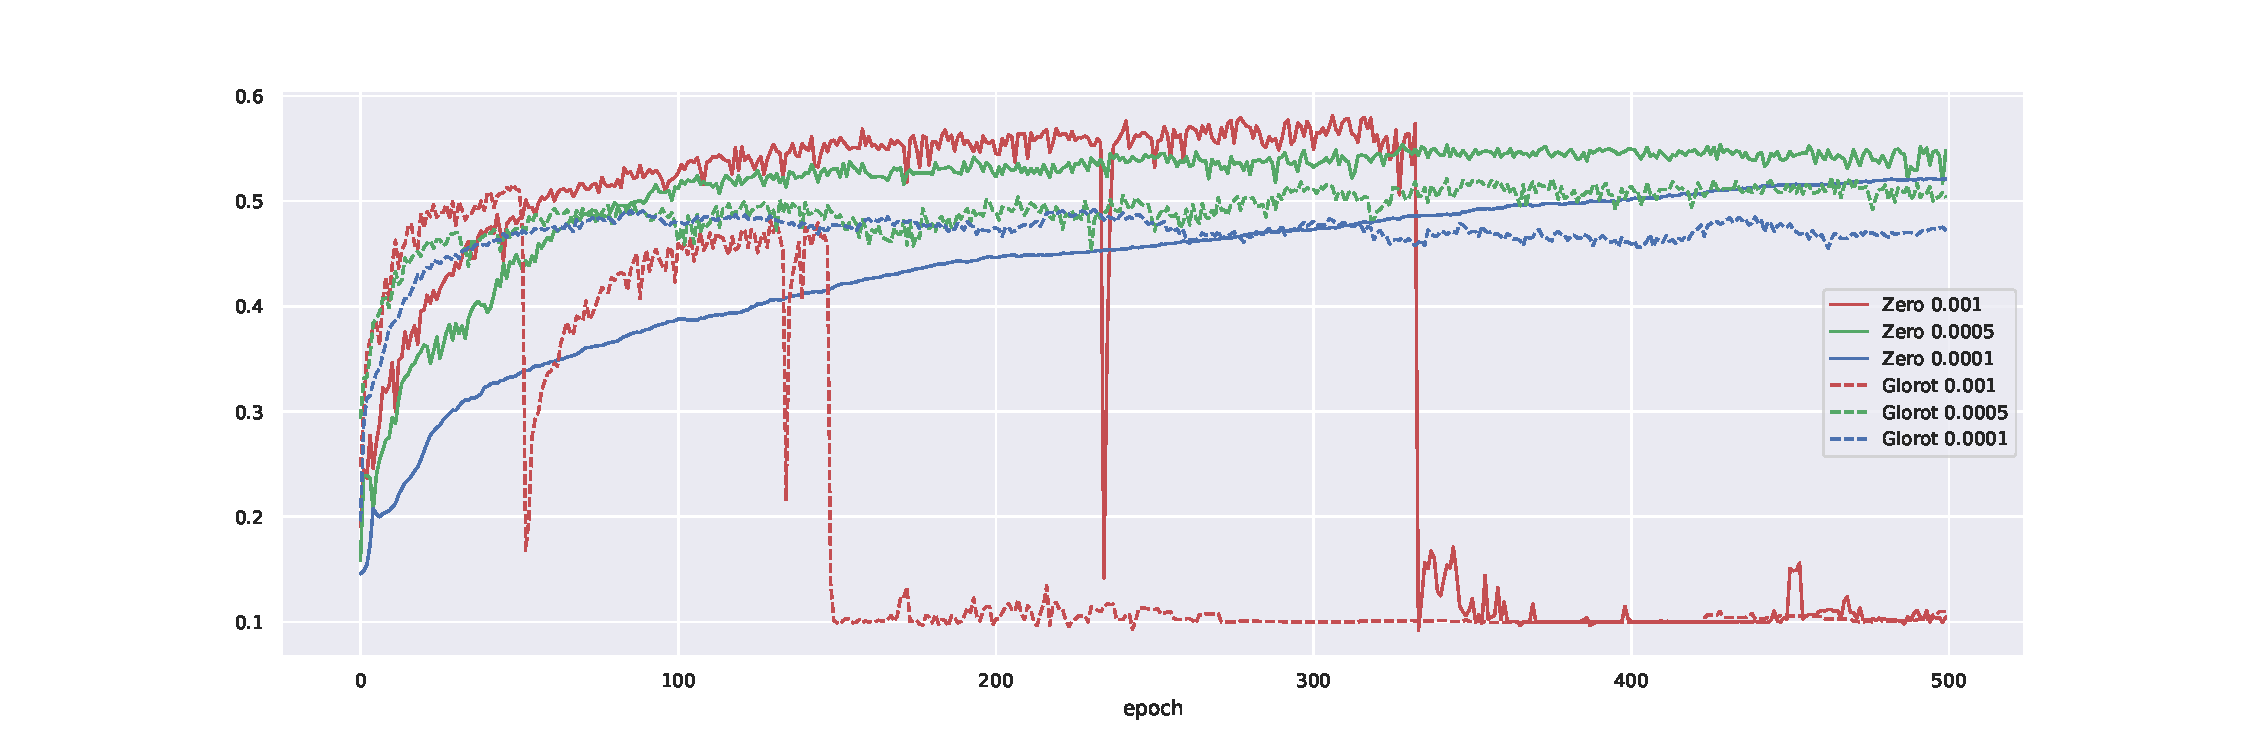
\includegraphics[width=1.0\textwidth]{zeros-vs-glorot}
\end{figure*}

\paragraph{Overfitting} Another interesting difference between Glorot and Zero initialization is the reduction of the gap between training and validation errors. Figure \ref{fig:ZeroVsGlorotDifference} show an histogram of differences between validation and training accuracies, where we can appreciate how Zero show smaller differences. 

\begin{figure}[h]\label{fig:ZeroVsGlorotDifference}
  \caption{Histogram of differences between train and validation accuracy.}
  \centering
    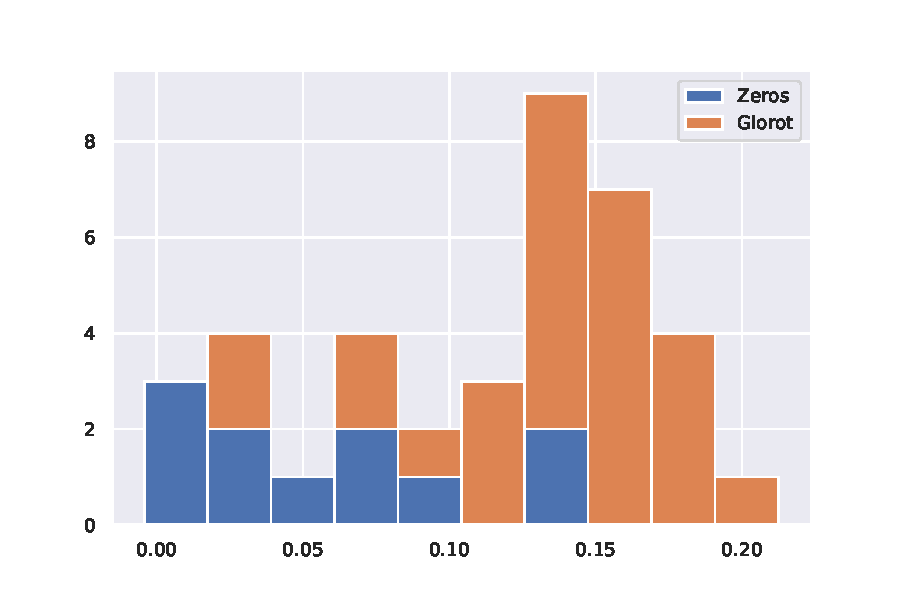
\includegraphics[width=0.5\textwidth]{zeros-vs-glorot-val-difference}
\end{figure}

\paragraph{Constraint loss} The following Figure \ref{fig:constraintLoss} show the accuracy achieved by each of the runs versus the loss from the constraints. We can see how having a low constraint loss is necessary but not sufficient condition for converging to good accuracy. We understand that this is proof of the importance of separability inside deep neural networks.

\begin{figure}[h]\label{fig:constraintLoss}
  \caption{Constraint loss vs accuracy in CIFAR-10.}
  \centering
    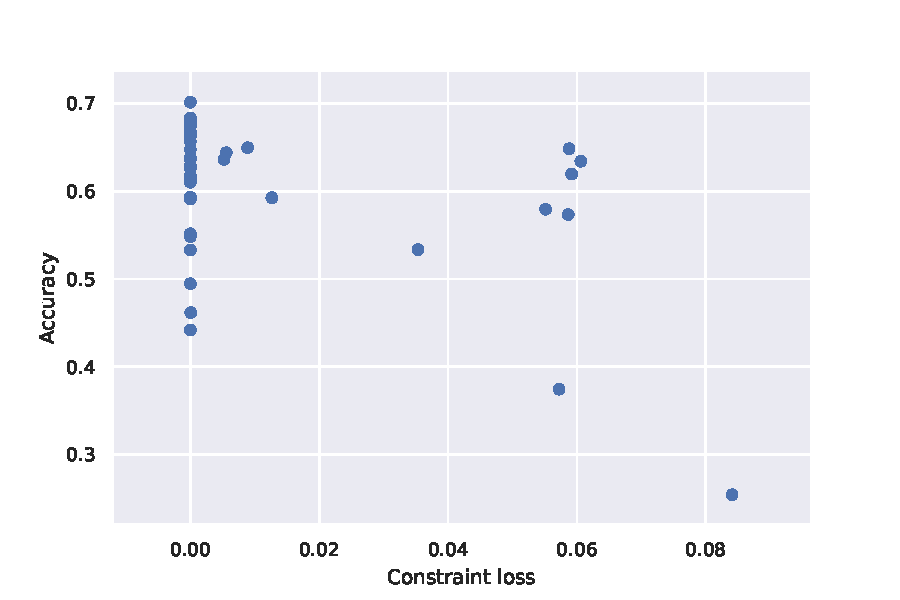
\includegraphics[width=0.5\textwidth]{constraint_loss}
\end{figure}


\paragraph{Lambda} We change $\lambda \in {0.00001,0.01000,1.00000}$ and freeze the rest of parameters and plot how the accuracy changes as $\lambda$ is increased at Figure \ref{fig:lambdas}. We separate Zeros and Glorot cases. We can see how increasing $\lambda$ is always translated to better performance. Notice also how the difference between training and validation accuracy grow when using Glorot.

\begin{figure}[h]\label{fig:lambdas}
  \caption{Accuracy versus Lambda.}
  \centering
    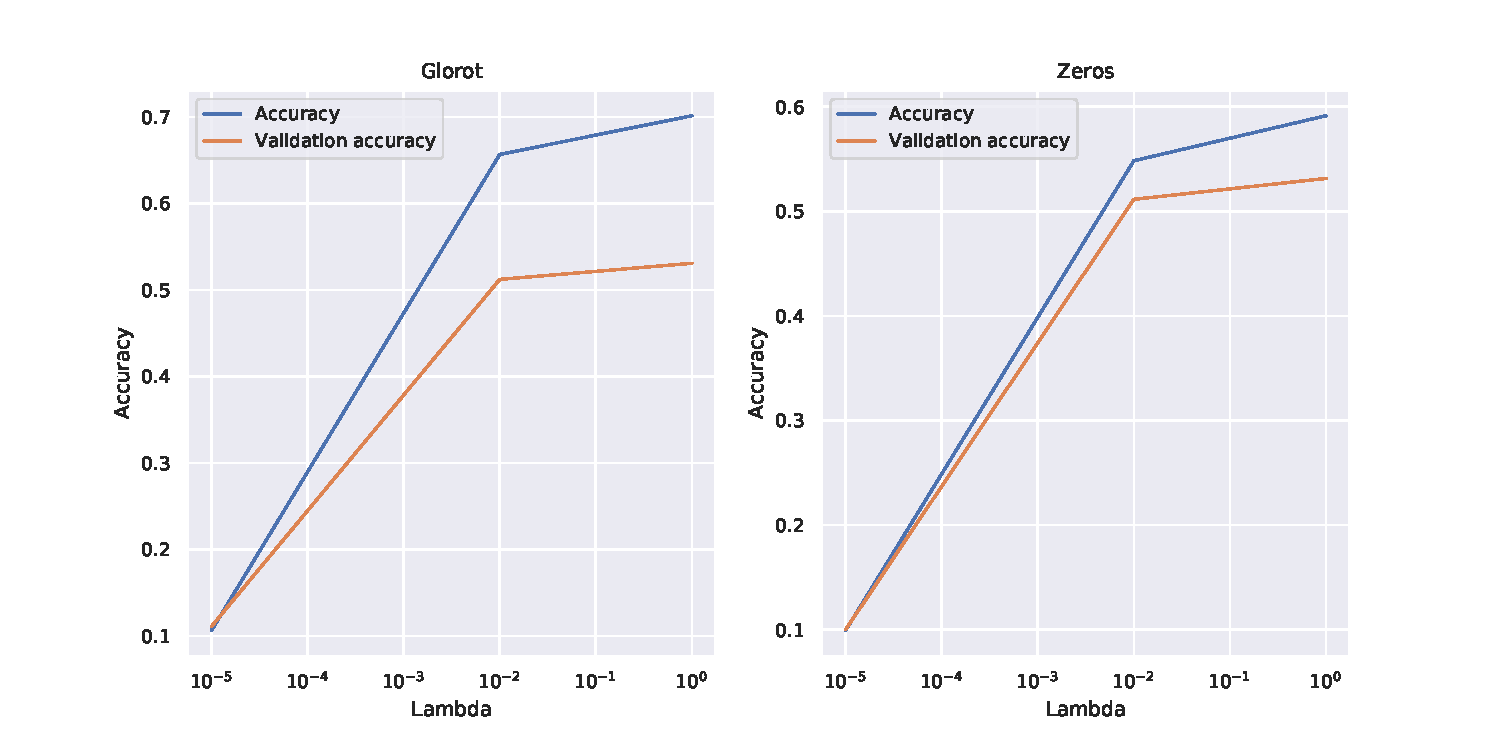
\includegraphics[width=0.5\textwidth]{lambdas}
\end{figure}

\subsection{Parameter and activation distribution}

We offer further proof of the actual suitability of our approach by presenting a figure containing the histograms of the activations and weights of a layer from the middle of the network, see Figure \ref{fig:histo}.
